\def\tutdate{1.12.2016}

\ifdefined\compileall \else
\ifdefined\compiletype
	\documentclass[handout]{beamer}
\else
	\documentclass{beamer}
	\def\compiletype{livebeamer}
\fi

\usepackage{templates/beamerthemekitwide}

\usepackage[utf8]{inputenc}
\usepackage[T1]{fontenc}
\usepackage[ngerman]{babel}
\usepackage{listings}
\usepackage{hyperref}
\usepackage{graphicx}

\usepackage{amsmath}
\usepackage{amsthm}
\usepackage{amssymb}
\usepackage{polynom}

\usepackage{ifthen}
\usepackage{adjustbox} % for \adjincludegraphics

\newcommand{\markBlue}[1]{\textcolor{kit-blue100}{#1}}
\newcommand{\markGreen}[1]{\textcolor{kit-green100}{#1}}

\newcommand{\pitem}{\pause\item}
\newcommand{\p}{\pause}

% -- MATH MACROS
\newcommand{\thistheoremname}{}
\newcommand{\G}{\mathbb{Z}}
\newcommand{\B}{\mathbb{B}}
\newcommand{\R}{\mathbb{R}}
\newcommand{\N}{\mathbb{N}}
\newcommand{\Q}{\mathbb{Q}}
\newcommand{\C}{\mathbb{C}}
\newcommand{\Z}{\mathbb{Z}}
\newcommand{\F}{\mathbb{F}}
\newcommand{\mi}{\mathrm{i}}
\renewcommand{\epsilon}{\varepsilon}


\newenvironment<>{taskblock}[1]{%
	\setbeamercolor{block title}{fg=kit-orange15,bg=kit-orange100}
	\setbeamercolor{block body}{fg=black,bg=kit-orange30}%
	\begin{block}#2{#1}}{\end{block}}

\setbeamertemplate{enumerate items}[default]

% Aussagenlogik Symbole
\newcommand{\W}{w}
\renewcommand{\F}{f}

% Kodierung
\newcommand{\frepr}{\textbf{repr}}
\newcommand{\fRepr}{\textbf{Repr}}
\newcommand{\fZkpl}{\textbf{Zkpl}}
\newcommand{\fbin}{\textbf{bin}}
\newcommand{\fdiv}{\textbf{ div }}
\newcommand{\fmod}{\textbf{ mod }}

\title[Grundbegriffe der Informatik]{Grundbegriffe der Informatik\\Tutorium 33}
\subtitle{}
\author{Lukas Bach, lukas.bach@student.kit.edu}
\date{\tutdate}

\institute{}

\titlelogo{lukasbach}

\titleimage{bg}
%\titleimage{bg-advent}


\ifthenelse{\equal{\compiletype}{livebeamer}}
	{
		\def\livebeamermode{1}
	}{}

\ifthenelse{\equal{\compiletype}{print}}
	{
		\def\printmode{1}
	}{}

\setbeamercovered{invisible}

%\usepackage[citestyle=authoryear,bibstyle=numeric,hyperref,backend=biber]{biblatex}
%\addbibresource{templates/example.bib}
%\bibhang1em

\begin{document}
	
\selectlanguage{ngerman}


%title page
\begin{frame}
	\titlepage
\end{frame}

%table of contents
\ifdefined\printmode
	\ifdefined\compileall \else
	\begin{frame}{Gliederung}
		\tableofcontents
	\end{frame}
\fi\fi

\fi

% Zur Anpassung: Dekommentiere folgende Zeilen, um weniger \pause zu haben
% \renewcommand{\ip}{} % inline pause, für mitten im satz

% Dekommentiere folgende Zeilen, um Stil besser an deine Folien anzupassen
%\renewenvironment{taskblock}[1]{\textbf{Aufgabe: #1}\\}{}
%\renewcommand{\markBlue}[1]{\textbf{#1}}
%\renewcommand{\markGreen}[1]{\textbf{#1}}

% begin of slides

\section{Zum Übungsblatt}

\begin{frame}{Anmerkungen zum letzten Übungsblatt}
	\begin{itemize}
		\pitem Was ist sind die folgenden Mengen?
		\begin{itemize}
			\pitem $\N$ \pause = Menge der natürlichen Zahlen (1, 2, 3, ...)
			\pitem $\N_0$ \pause = $\N \cup \{0\}$
			\pitem $\R$ \pause = Menge der Reellen Zahlen
			\pitem $\R^+$ \pause = Menge der positiven reellen Zahlen
			\pitem $\R_0$ \pause gibt es nicht! $0$ ist auch so schon in $\R$
			\pitem $\R_0^+$ genauso nicht!
		\end{itemize}
		\pitem Aufgabe: $R: A^* \rightarrow A^*$
		\begin{itemize}
			\item $R(\epsilon) = \epsilon$
			\item $\forall x \in A: R(x) = x$
			\item $\forall w \in A^* \forall x \in A \forall y \in A: R(xwy) = yR(w)x$
			\item Zeige: $\forall n \in \N_0 : \forall w \in A^n: |R(w)| = |w|$
		\end{itemize}
	\end{itemize}
\end{frame}

\section{MIMA}

\begin{frame}{Was ist die MIMA?}
	\begin{itemize}
		\pitem Theoretischer, idealisierter Prozessor
		\pitem Funktioniert wie ein echter Prozessor, ist aber simpler
		\pitem Nah an Technischer Informatik
	\end{itemize}

	\bp
	
	Grundaufbau:
	
	\begin{itemize}
		\pitem Adressen als $20bit$ Datenwort
		\pitem Speicherworte als $24bit$ Datenwort
		\pitem Maschinenbefehle als...
		\begin{itemize}
			\item $4bit$ Befehl und $20bit$ Adresse
			\item oder $8bit$ Befehl und unwichtigem Rest
		\end{itemize}
	\end{itemize}
\end{frame}

\begin{frame}{Aufbau der MIMA: Steuerwerk}
	\begin{center}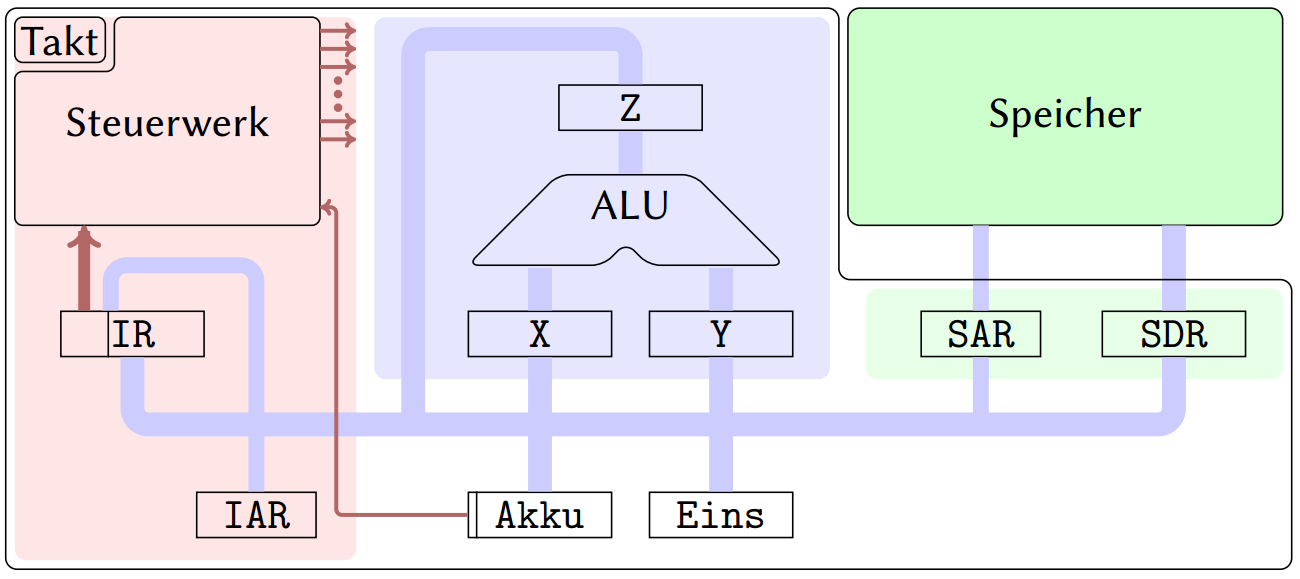
\includegraphics[width=.6\textwidth]{images/mima_aufbau.png}\end{center}
	
	\bp
	
	\textcolor{kit-red50}{\textbf{Steuerwerk}}
	
	\begin{columns}
		\begin{column}{0.5\textwidth}
			\begin{itemize}
				\pitem Instruction Register (IR) enthält den nächsten auszuführenden Befehl
				\pitem Instruction Adress Register (IAR) enthält die Adresse des nächsten Befehls
			\end{itemize}
		\end{column}
		
		\begin{column}{0.5\textwidth}
			\begin{itemize}
				\pitem Takt bestimmt die ``Tickrate'', also die Geschwindigkeit
				\pitem Steuerwerk interpretiert alle Befehle und führt sie aus
				\pitem Welche Befehle es gibt: Siehe später
			\end{itemize}
		\end{column}
	\end{columns}
	
\end{frame}


\begin{frame}{Aufbau der MIMA: Akku und Eins}
	\begin{center}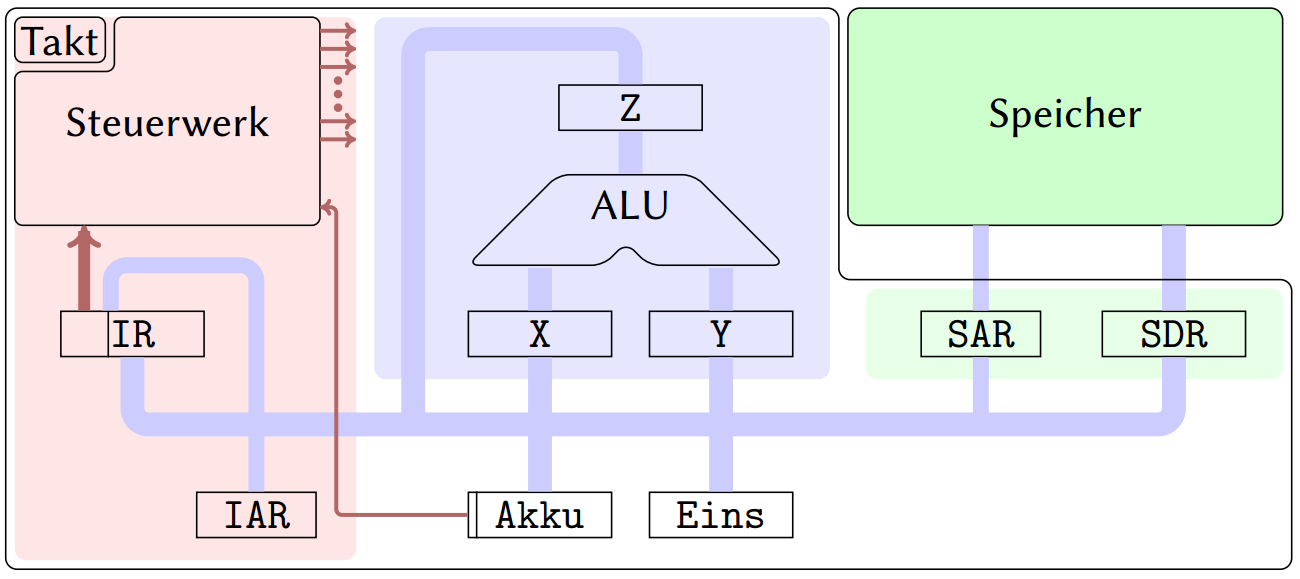
\includegraphics[width=.6\textwidth]{images/mima_aufbau.png}\end{center}
	
	\bp
	
	\textcolor{kit-orange50}{\textbf{Akku und Eins}}
	
	\begin{columns}
		\begin{column}{0.5\textwidth}
			\begin{itemize}
				\pitem Akku dient als Zwischenspeicher für Datenworte
				\pitem Hält maximal ein Wort
			\end{itemize}
		\end{column}
		
		\begin{column}{0.5\textwidth}
			\begin{itemize}
				\pitem Eins liefert die Konstante 1, hält also Strom
				\pitem z.B. erhöhen des IAR
			\end{itemize}
		\end{column}
	\end{columns}
	
\end{frame}


\begin{frame}{Aufbau der MIMA: ALU}
	\begin{center}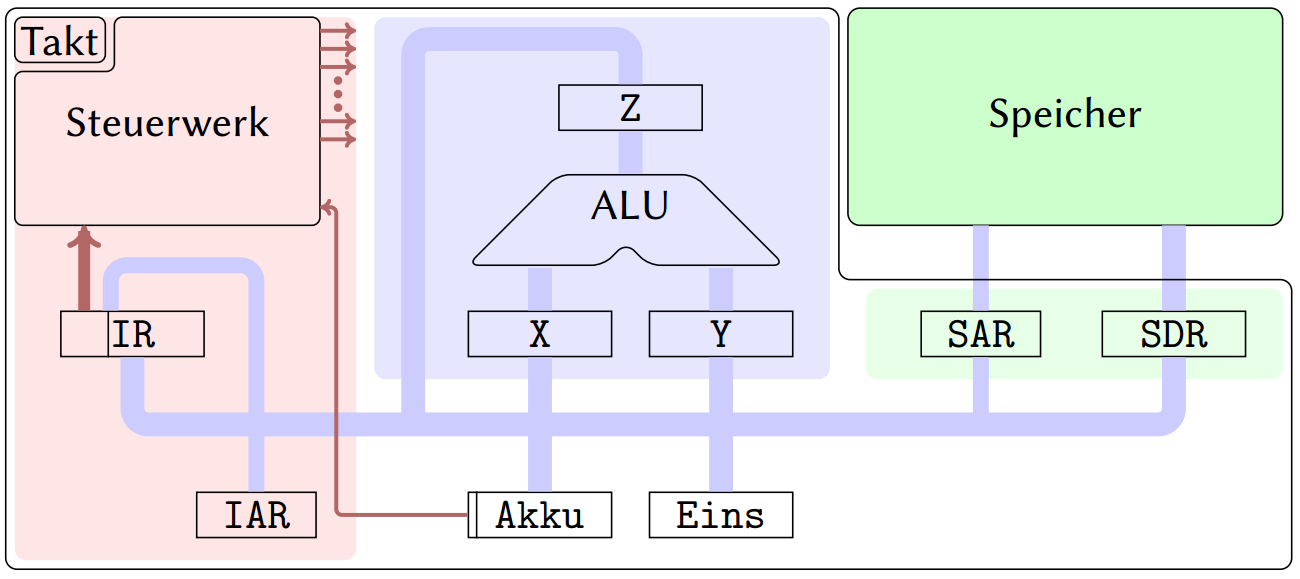
\includegraphics[width=.6\textwidth]{images/mima_aufbau.png}\end{center}
	
	\bp
	
	\textcolor{kit-blue50}{\textbf{Arithmetic Logic Unit (ALU) / Rechenwerk}}
	
	\begin{columns}
		\begin{column}{0.5\textwidth}
			\begin{itemize}
				\pitem Durchführt arithmetische Operationen
				\pitem $\fmod, \fdiv, +, -, ...$, bitweises OR/AND/...
			\end{itemize}
		\end{column}
		
		\begin{column}{0.5\textwidth}
			\begin{itemize}
				\pitem $X$ und $Y$ sind Eingaberegister
				\pitem $Z$ ist Ausgaberegister
			\end{itemize}
		\end{column}
	\end{columns}

\end{frame}


\begin{frame}{Aufbau der MIMA: ALU}
\begin{center}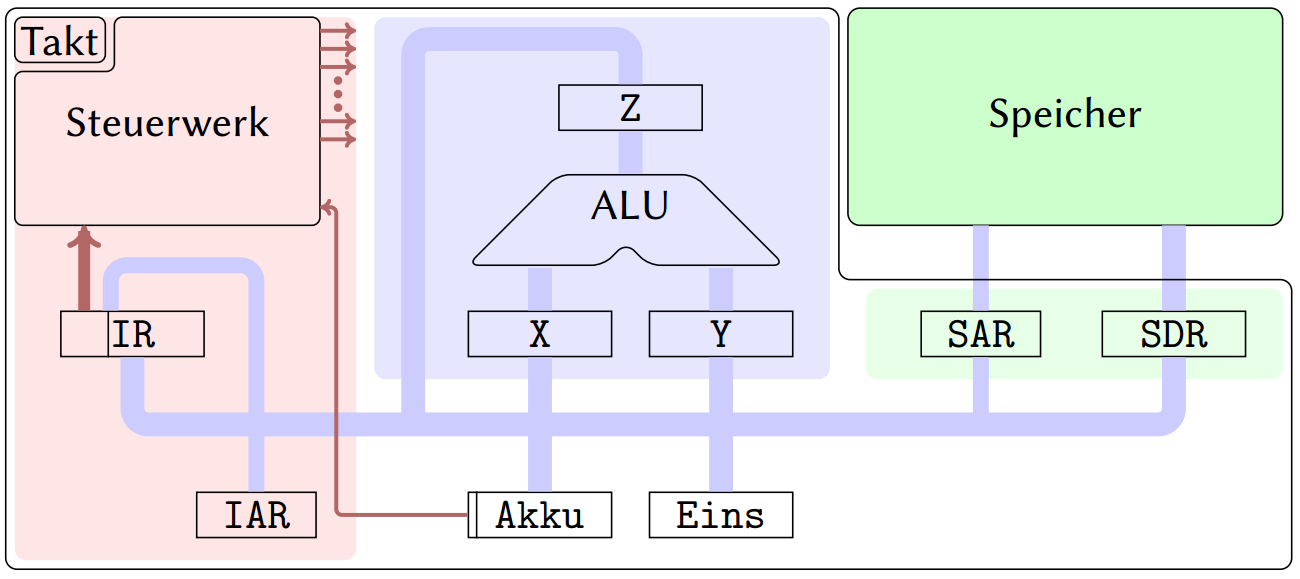
\includegraphics[width=.6\textwidth]{images/mima_aufbau.png}\end{center}

\bp

\textcolor{kit-green50}{\textbf{Speicher(werk)}}

Speicher selbst speichert Befehle und Daten. \ip Speicherwerk besteht aus:

\begin{columns}
	\begin{column}{0.5\textwidth}
		\begin{itemize}
			\pitem Speicheradressregister (SAR) ist die Adresse, bei der im Speicher gespeichert/gelesen werden soll
		\end{itemize}
	\end{column}
	
	\begin{column}{0.5\textwidth}
		\begin{itemize}
			\pitem Speicherdatenregister (SDR) Datum, das bei der Adresse gespeichert werden soll/ gelesen wurde.
		\end{itemize}
	\end{column}
\end{columns}

\end{frame}


\begin{frame}{Aufbau der MIMA: ALU}
\begin{center}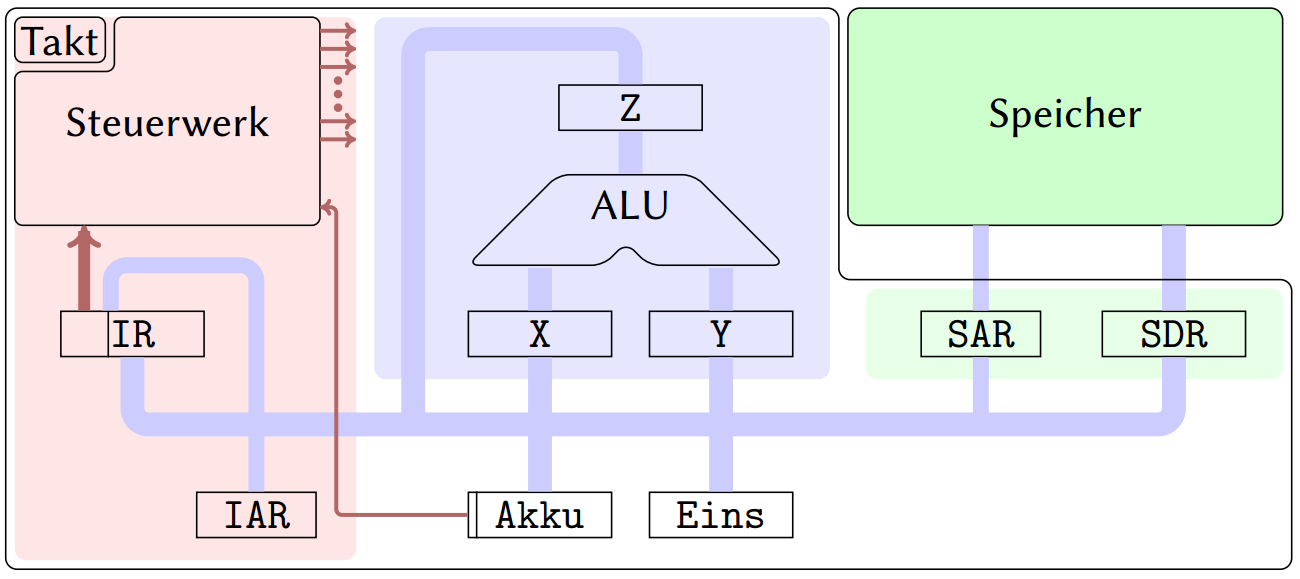
\includegraphics[width=.6\textwidth]{images/mima_aufbau.png}\end{center}

\bp

\textbf{Busse}

\begin{columns}
	\begin{column}{0.5\textwidth}
		\begin{itemize}
			\pitem ``Kabel'' zwischen den Verbindungen
			\pitem Ein kompletter Bus überträgt entweder $1$, $0$, oder nichts
		\end{itemize}
	\end{column}
	
	\begin{column}{0.5\textwidth}
		\begin{itemize}
			\pitem Kann nur eine einzige Information auf einmal übertragen
		\end{itemize}
	\end{column}
\end{columns}

\end{frame}

\begin{frame}{Konventionen zu MIMA Programmen}
	Um MIMA Programme und dazugehörige Definitionen verständlicher zu machen, vereinbaren wir folgende Konventionen:
	
	\bp
	
	\begin{itemize}
		\item Befehle (eigentlich Bitfolge) schreiben wir als Befehlname und Adresse
		\begin{itemize}
			\pitem $001000000000000000101010 \equiv STV 42$
		\end{itemize}
		\pitem $X \leftarrow Y \equiv $ ``Der Variable $X$ wird der Wert $Y$ zugewiesen''
		
	\end{itemize}
	
	
\end{frame}

\subsection{Maschinenbefehle}

% Folgende 3 Folien sollten nicht allzu ordentlich behandelt werden, mehr als vorzeitige Übersicht wieviele Befehle es gibt und als Referenz für die Tutanten für die Übungsaufgaben
\begin{frame}{MIMA Befehle}
	Eine MIMA-Maschine beherrscht folgende Maschinenbefehle:
	
	\vspace{.5cm}
	
	\begin{tabular}{r | l p{5cm} }
		Befehlssyntax & Formel & Bedeutung\\\hline\hline \ip
		$LDC$ $const$ & $Akku \leftarrow const$ & Lade eine Konstate $const$ in den Akku \\\hline \ip
		$LDV$ $adr$ & $Akku \leftarrow M(adr)$ & Lade einen Wert vom Speicher bei Adresse $adr$ in den Akku\\\hline\ip
		$STV$ $adr$ & $M(adr) \leftarrow Akku$ & Lade Speichere den Wert aus dem Akku im Speicher bei Adresse $adr$\\\hline\ip
		$LDIV$ $adr$ & $Akku \leftarrow M(M(adr))$ & Lade einen Wert vom Speicher bei der Adresse, die bei $adr$ gespeichert ist, und lade den Wert in den Akku\\\hline\ip
		$STIV$ $adr$ & $M(M(adr)) \leftarrow Akku$ & Speichere den Wert im Akku bei der Adresse, die in $adr$ gespeichert ist.
	\end{tabular}
\end{frame}

\begin{frame}{MIMA Befehle (2)}
	Eine MIMA-Maschine beherrscht folgende Maschinenbefehle:
	
	\vspace{.5cm}
	
	\begin{tabular}{r | l p{3cm} }
		Befehlssyntax & Formel & Bedeutung\\\hline\hline \ip
		$ADD$ $adr$ & $Akku \leftarrow Akku + M(adr)$ & Addiere den Wert bei $adr$ zum Akku dazu.\\\hline\ip
		$``OP''$ $adr$ & $Akku ``OP'' M(adr)$ & Wende bitweise Operation auf Akku mit Wert bei $adr$ an. $Op \in \{AND, OR, XOR\}$.
	\end{tabular}
\end{frame}

\begin{frame}{MIMA Befehle (3)}
	Eine MIMA-Maschine beherrscht folgende Maschinenbefehle:
	
	\vspace{.5cm}
	
	\begin{tabular}{r | p{8cm} }
		Befehlssyntax & Bedeutung\\\hline\hline \ip
		$NOT$ & Bitweise Invertierung aller Bits des Akku-Datenwortes\\\hline\ip
		$RAR$ & Rotiere alle Akku-Bits eins nach rechts\\\hline\ip
		$EQL$ $adr$ & Setze Akku auf $11\cdots11$, falls Wert bei $adr$ gleich Akku-Wert, setze Akku auf $00\cdots00$ sonst.\\\hline\ip
		$JMP$ $adr$ & Springe zu Befehlsadresse $adr$\\\hline\ip
		$JMN$ $adr$ & Springe zu Befehlsadresse $adr$, falls Akku negativ (also erstes Bit $=1$), sonst fahre normal fort.
	\end{tabular}
\end{frame}

% Bei folgenden Folien eventuell den Speicher auf die Tafel abschreiben und das Programm Befehl für Befehl durchgehen

% Laden und Speichern
\begin{frame}{MIMA Befehle: Sichern und Laden}
	\begin{itemize}
		\pitem Befehle zum laden und Speichern in den Speicher
		\pitem LDV um Daten vom Speicher zu laden, STV um Daten in den Speicher zu schreiben
		\pitem LDC um eine Konstante zu laden
		\pitem Daten werden in einem Zwischenspeicher gelagert, der nur ein Datenwort hält\ip : Akku.
	\end{itemize}

	\bp

	Beispiele:
	
	\begin{itemize}
		\pitem $LDV 9$ lädt das Datum, das im Speicher bei Adresse $9$ liegt, in den Akku.
		\pitem $STV 9$ speichert das Datum, das im Akku liegt, in den Speicher an Adresse $9$.
		\pitem $LDC 4$ lädt die Zahl $4$ in den Akku (also kein Speicherzugriff).
	\end{itemize}
\end{frame}

\begin{frame}{MIMA Befehle: Sichern und Laden}
	\begin{tabular}{r | l p{5cm} }
		Befehlssyntax & Formel & Bedeutung\\\hline\hline 
		$LDC$ $const$ & $Akku \leftarrow const$ & Lade eine Konstate $const$ in den Akku \\\hline 
		$LDV$ $adr$ & $Akku \leftarrow M(adr)$ & Lade einen Wert vom Speicher bei Adresse $adr$ in den Akku\\\hline
		$STV$ $adr$ & $M(adr) \leftarrow Akku$ & Lade Speichere den Wert aus dem Akku im Speicher bei Adresse $adr$\\\hline
	\end{tabular}

	\bp 
	\vspace{.5cm}
	\markGreen{Beispielprogramm mit initialem Speicherabbild}
	\vspace{.2cm}
	
	\begin{columns}
		\begin{column}{0.5\textwidth}
			LDC 5 \\ STV $a_1$ \\ LDC 7 \\ STV $a_2$ \\ LDV $a_1$ \\ STV $a_3$ \\ HALT
		\end{column}
		
		\begin{column}{0.5\textwidth}
			\begin{memory}
				\memrow{$a_1$}{0}	
				\memrow{$a_2$}{0}
				\memrow{$a_3$}{0}
			\end{memory}
		\end{column}
	\end{columns}

	%TODO Ergebnis
\end{frame}

% Laden und Speichern (indirekt)
\begin{frame}{MIMA Befehle: Indirektes Sichern und Laden}
	\begin{tabular}{r | l p{5cm} }
		Befehlssyntax & Formel & Bedeutung\\\hline\hline 
		$LDIV$ $adr$ & $Akku \leftarrow M(M(adr))$ & Lade einen Wert vom Speicher bei der Adresse, die bei $adr$ gespeichert ist, und lade den Wert in den Akku\\\hline
		$STIV$ $adr$ & $M(M(adr)) \leftarrow Akku$ & Speichere den Wert im Akku bei der Adresse, die in $adr$ gespeichert ist.
	\end{tabular}
	
	\bp 
	\vspace{.5cm}
	\markGreen{Beispielprogramm mit initialem Speicherabbild}
	\vspace{.2cm}
	
	\begin{columns}
		\begin{column}{0.5\textwidth}
			LDIV 4 \\ STV 5 \\ LDIV 5 \\ STIV 4 \\ HALT
		\end{column}
		
		\begin{column}{0.5\textwidth}
			\begin{memory}
				\memrow{$4$}{$6$}	
				\memrow{$5$}{$0$}
				\memrow{$6$}{$7$}
				\memrow{$7$}{$2$}
			\end{memory}
		\end{column}
	\end{columns}
\end{frame}

% Arithmetische Operationen
\begin{frame}{MIMA Befehle: Eins plus Eins}
	\begin{itemize}
		\pitem Befehle zu arithmetischen Operationen
		\pitem Eine ALU-Operation, angewandt auf dem Wert des Akkus und dem Wert an gegebener Adresse
		
		\bp
		
		\item Beispiele:
		\begin{itemize}
			\pitem $ADD 4$ addiert den Wert im Akku mit dem Wert aus dem Speicher an Adresse $4$ und legt das Resultat im Akku ab\ip . Achtung: Addition nicht mit dem Wert $4$!
			\pitem $AND 3$ führt bitweise Verundung zwischen dem Wert im Akku und dem Wert aus dem Speicher an Adresse $4$ durch und legt das Resultat im Akku ab.
		\end{itemize}
	\end{itemize}
\end{frame}


\begin{frame}{MIMA Befehle: Eins plus Eins}
	\begin{tabular}{r | l p{5cm} }
		Befehlssyntax & Formel & Bedeutung\\\hline\hline 
		$ADD$ $adr$ & $Akku \leftarrow Akku + M(adr)$ & Addiere den Wert bei $adr$ zum Akku dazu.\\\hline
		$``OP''$ $adr$ & $Akku ``OP'' M(adr)$ & Wende bitweise Operation auf Akku mit Wert bei $adr$ an. $Op \in \{AND, OR, XOR\}$.
	\end{tabular}
	
	\bp 
	\vspace{.5cm}
	\markGreen{Beispielprogramm mit initialem Speicherabbild}
	\vspace{.2cm}
	
	\begin{columns}
		\begin{column}{0.5\textwidth}
			LDC 5 \\ ADD 3 \\ AND 4 \\ STV 5 \\ LDC 12 \\ XOR 5 \\ HALT
		\end{column}
		
		\begin{column}{0.5\textwidth}
			\begin{memory}
				\memrow{$3$}{$3$}	
				\memrow{$4$}{$8$}
				\memrow{$5$}{$17$}
			\end{memory}
		\end{column}
	\end{columns}
\end{frame}

% Logische Operationen
\begin{frame}{MIMA Befehle: Bits und Bytes }
	\begin{itemize}
		\pitem $NOT$ invertiert alle Bits des Datums im Akku. \ip Beispiel $NOT$ mit $5$ im Akku, angenommen der Akku speichert bis zu 8 bits\ip : $5_{10} = 00000101_2$, nach der Invertierung: $1111 1010_2$.
		
		\pitem $RAR$ rotiert alle Bits des Datums im Akku um eine Stelle nach rechts. \ip Beispiel mit $5$ im Akku: $00000\markBlue{101}_2$ wird zu $000000\markBlue{10}_2$.
		
		\pitem $EQL adr$ vergleicht den Wert im Akku mit dem Wert bei $addr$.
		\begin{itemize}
			\pitem Setzt Akku $= 11\cdots 11$ falls Werte gleich sind.
			\pitem Setzt Akku $= 00\cdots 00$ falls Werte nicht gleich sind.
		\end{itemize}
	\end{itemize}
\end{frame}
	
\begin{frame}{MIMA Befehle: Bits und Bytes }
	\begin{tabular}{r | p{8cm} }
		Befehlssyntax & Bedeutung\\\hline\hline 
		$NOT$ & Bitweise Invertierung aller Bits des Akku-Datenwortes\\\hline
		$RAR$ & Rotiere alle Akku-Bits eins nach rechts\\\hline
		$EQL$ $adr$ & Setze Akku auf $11\cdots11$, falls Wert bei $adr$ gleich Akku-Wert, setze Akku auf $00\cdots00$ sonst.\\\hline
	\end{tabular}
	
	\bp 
	\vspace{.5cm}
	\markGreen{Beispielprogramm mit initialem Speicherabbild}
	\vspace{.2cm}
	
	\begin{columns}
		\begin{column}{0.5\textwidth}
			LDC 5 \\ NOT \\ RAR \\ NOT \\ RAR \\ RAR \\ EQL 15 \\ EQL 0 \\ HALT
		\end{column}
		
		\begin{column}{0.5\textwidth}
		\end{column}
	\end{columns}
\end{frame}

% Programmstruktur Operationen
\begin{frame}{MIMA Befehle: Springen}
	\begin{itemize}
		\pitem Normalerweise wird die Instruktionsadresse nach jedem Befehl um eins erhöht
		\pitem Also Befehle werden von oben nach unten abgearbeitet
		\pitem Mit Sprüngen kann man die MIMA zwingen, zu definiertem Befehl zu springen und damit die Vorgehensreihenfolge zu beeinflussen
		
		\vspace{.3cm} \bp
		
		\item $JMP adr$ führt als nächsten Befehl den an Adresse $adr$ aus.
		\pitem $JMN adr$ führt als nächsten Befehl den an Adresse $adr$ aus, \markGreen{falls der Akku negativ ist}.
		\begin{itemize}
			\pitem Also wenn das erste Bit im Akku negativ ist.
			\pitem Wenn vorher ein $EQL$ erfolgreich verglichen hat, wird also gesprungen.
			\pitem Wenn der Akku positiv ist, werden die Befehle nach $JMN$ normal weiter abgearbeitet.
		\end{itemize}
	\end{itemize}
\end{frame}
	
\begin{frame}{MIMA Befehle: Springen}
	\begin{tabular}{r | p{8cm} }
		Befehlssyntax & Bedeutung\\\hline\hline 
		$EQL$ $adr$ & Setze Akku auf $11\cdots11$, falls Wert bei $adr$ gleich Akku-Wert, setze Akku auf $00\cdots00$ sonst.\\\hline
		$JMP$ $adr$ & Springe zu Befehlsadresse $adr$\\\hline
		$JMN$ $adr$ & Springe zu Befehlsadresse $adr$, falls Akku negativ (also erstes Bit $=1$), sonst fahre normal fort.
	\end{tabular}
	
	\bp 
	\vspace{.5cm}
	\markGreen{Beispielprogramm mit initialem Speicherabbild}
	\vspace{.0cm}
	
	\begin{columns}
		\begin{column}{0.5\textwidth}
			\begin{align*}
				& \text{LDC 5} \\
				a_1: \quad  & \text{JMN } a_2 \\
				& \text{EQL 1} \\
				& \text{JMN } a_1 \\
				& NOT \\ % sollte nicht erreicht sein
				a_2: \quad & \text{JMP } a_3\\
				& NOT \\ % sollte nicht erreicht sein
				a_3: \quad & HALT
			\end{align*}
		\end{column}
		
		\begin{column}{0.5\textwidth}
			\begin{memory}
				\memrow{$1$}{$5$}	
			\end{memory}
		\end{column}
	\end{columns}
\end{frame}

\subsection{Aufgaben}

\begin{frame}{Aufgaben}
	\begin{taskblock}{MIMA-Programm schreiben}
		Schreibe ein MIMA-Programm:
		\begin{itemize}
			\item Eingabe: Adresse $a_1$ einer positiven Zahl $x$.
			\item Ausgabe: Speichert $x \fmod 2$ in $a_1$.
		\end{itemize}
	\end{taskblock}

	\bp \vspace{.5cm} Lösung:
	
	LDC 1 \quad // 000000000000000000000001 \\ AND $a_1$ \\ STV $a_1$ \\ HALT
\end{frame}

\ifdefined\compileall
\else


\ifthenelse{\equal{\compiletype}{print}}
{

\begin{frame}{Informationen}
	
	\begin{columns}
		\begin{column}{0.5\textwidth}
			
			\begin{block}{Zum Tutorium}
				\begin{itemize}
					\item Lukas Bach
					\item Tutorienfolien auf: 
					\begin{itemize}
						\item \url{http://gbi.lukasbach.com}
					\end{itemize}
					\item Tutorium findet statt:
					\begin{itemize}
						\item Donnerstags, 14:00 - 15:30
						\item 50.34 Informatikbau, -107
					\end{itemize}
				\end{itemize}
			\end{block}
			
			\begin{block}{Mehr Material}
				\begin{itemize}
					\item Ehemalige GBI Webseite:
					\begin{itemize}
						\item \url{http://gbi.ira.uka.de}
						\item Altklausuren!
					\end{itemize}
				\end{itemize}
			\end{block}
			
		\end{column}
		\begin{column}{0.5\textwidth}
			
			\begin{block}{Zur Veranstaltung}
				\begin{itemize}
					\item Grundbegriffe der Informatik
					\item Klausurtermin:
					\begin{itemize}
						\item 06.03.2017, 11:00
						\item Zwei Stunden Bearbeitungszeit
						\item 6 ECTS für Informatiker und Informationswirte, 4 ECTS für Mathematiker und Physiker
					\end{itemize}
				\end{itemize}
			\end{block}
			
			\begin{block}{Zum Übungsschein}
				\begin{itemize}
					\item Übungsblatt jede Woche
					\item Ab 50\% insgesamt hat man den Übungsschein
					\item Keine Voraussetzung für die Klausur, aber für das Modul
				\end{itemize}
			\end{block}
			
		\end{column}
	\end{columns}
	
\end{frame}

}{}

\ifdefined\livebeamermode
	\begin{frame}
		
\includegraphics[width=\linewidth]{images/thatsall.png}
	\end{frame}
\fi

\end{document}

\fi